\section{Related Work}
\label{sec:related-work}

\epigraph{
    ``Not everyone in a society fits the cultural pattern precisely, but there is enough statistical regularity to identify trends and tendencies.''
}{
    Aaron Marcus and Emilie W. Gould~\cite{Marcus2010}
}

This chapter reviews the existing literature relevant to this thesis to address the research questions specified in \cref{sec:intro-research-question}.
It compiles prior research across various subject areas that, when considered together, delineate the scope of this thesis, identifying both its boundaries and its core areas of focus.
This collection is intentionally extensive, as the aim of this thesis is to establish a foundation for future research that benefits from situating the broader context in perspective.

First, this chapter outlines how human cultures can be scientifically differentiated.
The values embedded within these cultures lead us to observations on human behavior, particularly in terms of website interactions as users and website creation as software developers.
The chapter then examines code styles that researchers have linked to potential authors as well as technical features of product design introduced in response to globally varying user demands.
Understanding why certain methods are employed in product design and how statistics are formed on code authorship enables us to identify features for which we aim to discover global patterns in this thesis.

In the second section, this chapter identifies publicly available datasets that can be used to initiate our research on global variations in website code.
Additionally, some strategies for autonomous data sourcing are presented as complementary recommendations.

Finally, the combination of knowledge on analytical methods and accessible data will be enhanced by references to research on Big Data and data engineering.
This will allow us to propose a Big Data pipeline design to accomplish the primary objective of this thesis.


\subsection{Cultural Influence on Code}
\label{sec:related-work-culture}

Understanding cultural influence on code allows us to address \Cref{rq:1} of this thesis and thereby determine which feature patterns to focus on in our analysis.
Scientific evidence for cultural influence on code would encourage us to develop hypotheses on relationships between cultural values and styles of web development, which we could then seek to validate using our Big Data pipeline.
In the absence of such evidence, we would still be able to analyze certain feature patterns, though without attributing them to cultural influence.
Other motivations for analyzing feature patterns in website code include identifying security vulnerabilities, tracking web development trends, collecting metadata on network reliability, and more.

\subsubsection{Hofstede's Cultural Dimensions Theory}
\label{sec:related-work-culture-hofstede}

A frequently cited work on the topic of cultural values and corresponding behaviors is \textbf{Hofstede}'s cultural dimensions theory.
The original version of Hofstede's theory, introduced in his book \textit{Culture's Consequences: International Differences in Work-Related Values} (1984), featured four dimensions, which are explained in the following paragraph: \textit{Power Distance}, \textit{Individualism vs. Collectivism}, \textit{Masculinity vs. Femininity}, and \textit{Uncertainty Avoidance}~\cite{Hofstede1984}.
These dimensions were derived from a study of IBM employees and represent cultural values predominant in different countries.
Later, in 2001, Hofstede expanded the model by adding one more dimension in an updated version of his book titled \textit{Culture's Consequences: Comparing Values, Behaviors, Institutions and Organizations Across Nations}: \textit{Long-Term Orientation vs. Short-Term Orientation}~\cite{Hofstede2001}.
The final addition to Hofstede's dimensions, \textit{Indulgence vs. Restraint}, was included in the book \textit{Cultures and Organizations: Software of the Mind} in 2010, in collaboration with \textbf{Minkov}~\cite{Hofstede2010}.

\begin{enumerate}
    \item \textbf{\ac{pdi}} refers to the extent to which less powerful members of organizations and institutions accept and expect that power is distributed unequally.

    \item \textbf{\ac{idv}} examines whether people prefer to take care of themselves and their immediate family only or belong to tightly-knit communities that look after each other in exchange for loyalty.

    \item \textbf{\ac{mas}}\footnote{\ac{mas} was formerly known as \textbf{Masculinity vs. Femininity}.} explores the distribution of roles between genders as assumed by Hofstede: Masculine societies value competitiveness, assertiveness, ambition, and the accumulation of wealth and material possessions, while feminine societies place more value on relationships and quality of life.

    \item \textbf{\ac{uai}} measures tolerance for uncertainty and ambiguity within society.
    Cultures with high \ac{uai} scores have strict rules and regulations, while those with low \ac{uai} scores are more relaxed.

    \item \textbf{\ac{lto}} distinguishes societies that are future-oriented and value persistence and thrift from those focused on the past and present, valuing traditions and social obligations.

    \item \textbf{\ac{ind}} refers to the extent to which a society allows relatively free gratification of basic and natural human drives related to enjoying life and having fun, as opposed to a society that suppresses gratification of needs and regulates it by means of strict social norms.
\end{enumerate}

A cultural analytics and strategy advisory from Finland, \textit{The Culture Factor Group}, offers the \textit{Country Comparison tool}, which allows comparison of the dimension values of several countries and regions~\cite{CFG2024}.
Continuing with the example introduced in \cref{sec:intro-background-and-motivation}, and by using the comparison tool, we can compare the index values for Germany and Japan in \cref{fig:country-comparison}.

\begin{figure}[H]
    \centering
    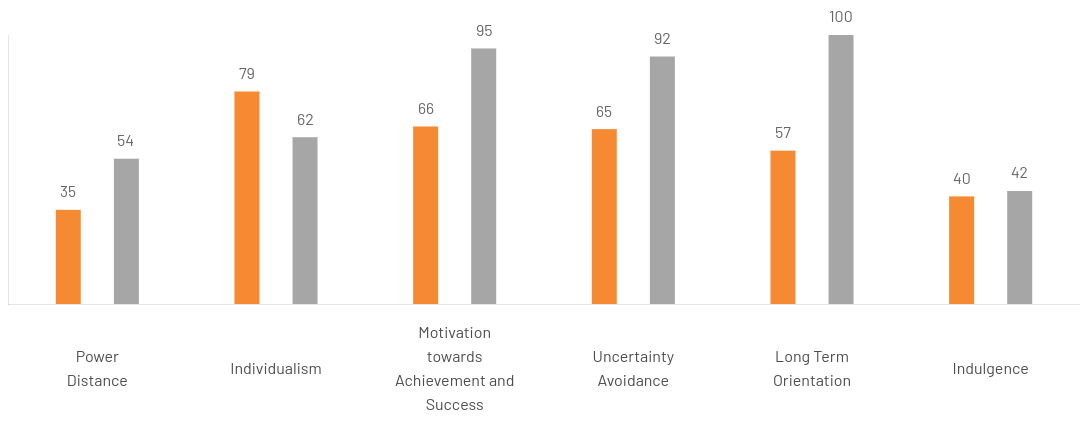
\includegraphics[width=\textwidth]{figures/country-comparison.png}
    \caption{Comparison of Hofstede's cultural dimension values for Germany (orange) and Japan (gray)~\cite{CFG2024}.}
    \label{fig:country-comparison}
\end{figure}

The comparison tool also provides explanations for the index values\footnote{The descriptions for all other index values are listed in \cref{sec:appendix-country-comparison-tool-descriptions}.}. Germany's \ac{pdi}, for example, is described as follows:

\begin{quote}
    ``Highly decentralised and supported by a strong middle class, Germany is not surprisingly among the lower power distant countries (score 35).
    Co-determination rights are comparatively extensive and have to be taken into account by the management.
    A direct and participative communication and meeting style is common, control is disliked, and leadership is challenged to show expertise and is best accepted when based on it.''~\cite{CFG2024}
\end{quote}

Japan's higher \ac{pdi} value, on the other hand, is explained as follows:

\begin{quote}
    ``At an intermediate score of 54, Japan is a borderline hierarchical society.
    Yes, Japanese are always conscious of their hierarchical position in any social setting and act accordingly.
    However, it is not as hierarchical as most of the other Asian cultures.
    Some foreigners experience Japan as extremely hierarchical because of their business experience of painstakingly slow decision making process: all the decisions must be confirmed by each hierarchical layer and finally by the top management in Tokyo.
    Paradoxically, the exact example of their slow decision making process shows that in Japanese society there is no one top guy who can take decision like in more hierarchical societies.
    Another example of not so high Power Distance is that Japan has always been a meritocratic society.
    There is a strong notion in the Japanese education system that everybody is born equal and anyone can get ahead and become anything if he (yes, it is still he) works hard enough.''~\cite{CFG2024}
\end{quote}

There is considerable psychological evidence supporting the accuracy of Hofstede's findings.
For example, \textit{taijin kyofusho} is described as a ``Japanese form of social anxiety'' by \textbf{Essau et al.} (2011), summarized as an ``intense fear that one's body parts or functions displease, embarrass, or are offensive to others''~\cite{Essau2011}.
This anxiety can be seen as a contributing factor to Japan's high \ac{uai} score of 92.

Hofstede's country-based distinctions have faced criticism, with some arguing that they constitute an unjust separation.
A notable paper addressing the issue of national culture was published by \textbf{Witte} (2011).
In \textit{Making the Case for a Post-national Cultural Analysis of Organizations}, Witte argues that ``Postcolonial theory has revealed that research paradigms promoting gender, nation, age, ethnic, and other categories suffer from bias implicit in all 'essentializing' and 'reifying' projects''~\cite{Witte2011}.

A similar critique is raised by \textbf{Cater-Steel and Toleman} (2008), who highlight that, as part of the globalization of software engineering, development tasks are frequently outsourced to countries offering lower labor costs, and IT professionals increasingly migrate internationally~\cite{Steel2008}.
To assess the current state of software engineering's globalization and related cultural differences in developer behavior, the following section examines the impacts of \ac{gse} more closely.


\subsubsection{\acl{gse}}
\label{sec:related-work-culture-gse}

Research on the globalization of software development, beginning in the early 2000s, points to a growing trend of software components being developed in countries other than those where the organizations distributing the composite software product are based.
Early studies, such as those by \textbf{J. S. Olson and G. M. Olson} (2003)~\cite{Olson2003} and \textbf{Abraham} (2009)~\cite{Abraham2009}, cautiously observe the emerging effects of globalization on software development.

Around 2010, scientific articles began critically examining the exploitative nature of outsourced development work, as highlighted by \textbf{Patel et al.} (2009)~\cite{Patel2009} and \textbf{Casey} (2009)~\cite{Casey2009}, along with the risks associated with international teams, such as communication conflicts due to language barriers, as modeled by \textbf{Wattanapokasin and Rivepiboon} (2009)~\cite{Wattanapokasin2009}.

A few years later, these risks were framed more directly in publications such as \textit{Cultural Characteristics and Their Connection to Increased Risk of Software Project Failure} by \textbf{Jørgensen and Yamashita} (2016)~\cite{Joergensen2016}.
Cultural barriers appear to have been higher than anticipated, leading to increased costs for companies that chose to outsource some of their labor.

These observations led to more actionable guidance, such as the suggestion to conduct onsite visits as one of twelve \textit{Practices for Cultural Differences} laid out by \textbf{Marinho et al.} (2018)~\cite{Marinho2018} and the \textit{Conversational Agent for the Detection Of Community Smells} proposed as a ``framework [...] for immediate application'' by \textbf{Lambiase} (2024)~\cite{Lambiase2024}.

Corporate-level development is often not the first point of intercultural collaboration for software developers, however.
For instance, \textbf{Hoda et al.} (2017) identified socio-cultural challenges in \ac{gsee} for educators and students, including a varying concept of time and attitude towards grades~\cite{Hoda2017}.

A study by \textbf{Shah and Harrold} (2013) specifically focused on behavioral differences in coding practices among developers from different countries.
The study identified differences in testing depth, time management, as well as expectations and perceptions of quality.
While a team based in Japan prioritized thorough testing of error-prone scenarios, a team based in the United States of America focused more on ensuring functionality and efficiency in frequently used features.
Furthermore, the Japanese team showed greater reluctance toward outsourcing testing~\cite{Shah2013}, which may correlate with Japan's high \ac{uai} score.

If variations in testing approaches are influenced by cultural nuances, it can be assumed that other coding practices, such as code structuring and formatting, are likely subject to the same influence.
When considered as a whole, it is conceivable that identifiable traces of cultural influence in the code could allow conclusions about the origin of code authorship.
Consequently, the following section summarizes significant publications on the traceability of code ownership.


\subsubsection{Fingerprinting}
\label{sec:related-work-culture-fingerprinting}

Having explored the cultural impacts on human interaction in software engineering, one question remains: Is it possible to draw conclusions about software authors merely by examining their code?
This question has driven many researchers to experiment with public datasets, aiming to de-anonymize programmers for various purposes.

A pivotal study by \textbf{Caliskan-Islam et al.} (2015) achieved an accuracy of 94\% in attributing code to 1,600 authors using a C/C++ code style dataset~\cite{CaliskanIslam2015}.
This author count is significantly higher than in earlier experiments, where studies commonly involved fewer than 50 authors, or even as few as 10.
The increased accuracy with larger author pools was enabled by analyzing \acp{ast}.
Previous research mostly relied on less structured data, such as the frequencies of code tokens like \texttt{if} and \texttt{for} statements.
Caliskan-Islam et al. also observed that difficult programming tasks tend to yield higher accuracy in code attribution, whereas less skilled programmers are harder to attribute, regardless of task difficulty.

A notable aspect of Caliskan-Islam et al.'s study is that it maintained high accuracy even for obfuscated code, which is neither human-readable nor maintainable.
The C++ obfuscator \textit{stunnix} reduced authorship identification accuracy from 100\% to 98.89\% for 20 programmers, only a 1.11 percentage point decrease.
A more thorough C obfuscator, \textit{Tigress}, which can specialize the bytecode of functions\footnote{Tigress calls this \textit{function virtualization}: \url{https://tigress.wtf/virtualize.html}}, lowered the identification accuracy from 93.65\% to 58.33\%, a reduction of 35.32\%.

A noteworthy 2006 study provides historical context for the achievements of Caliskan-Islam et al. by identifying recurring patterns in software code through an innovative compression-based approach.
\textbf{Gil et al.} used the compression mechanism of one large program to compress another and judged program similarity based on compression ratio differences.
Programs with similar patterns had similar compression ratios, suggesting a higher likelihood of common authorship.
However, this method did not reliably identify authors, as it could only infer relative relationships~\cite{Gil2006}.

One year later, in 2007, \textbf{Lange and Mancoridis} introduced a similarly innovative approach to software authorship identification, using genetic algorithms to optimize combinations of code style metrics that distinguished likely authors of code files from a candidate pool.
They interpreted 18 code style metrics as ``genes'', with varying combinations representing ``organisms'', which in turn formed ``populations'' that evolved across generations, strengthening or weakening as they adapted~\cite{Lange2007}.

This genetic algorithm developed by Lange and Mancoridis resembles \ac{nn} training but was proposed roughly a decade before the rise of \ac{ml}.
Unlike \acp{nn}, which assign individual weights to each input, genetic encoding produces a Boolean combination of selected features.

All code style metrics in Lange and Mancoridis' research can be categorized as tokenized metrics.
Brace positions, indentation style, and line lengths can be determined through character-wise parsing without requiring computationally intensive structures like \acp{ast}.

In 2019, \textbf{Gorshkov et al.} followed this lineage with their study on \textit{Using Machine Learning Methods to Establish Program Authorship}.
They addressed the complexities of collaborative software development in a globalized context, setting their work apart by tackling authorship identification in files with multiple authors, where authorship boundaries within files are unknown.
They argued that their \ac{ml} methods detect the use of programming paradigms that can suggest developers' expertise levels.
According to Gorshkov et al., code written by non-experts can then be automatically synthesized with expert code to improve overall code quality.
The following four areas were identified in Gorshkov et al.'s journal article as characteristic of programming styles:

\begin{enumerate}
    \item General programming practices, such as rules and recommendations,
    \item typographic styles, such as the use of comments,
    \item control structure styles, such as algorithm choice, and
    \item information structure styles, such as data storage decisions~\cite{Gorshkov2019}.
\end{enumerate}

Within the same year, \textbf{Mahbub et al.} (2019) took a similar approach to Gorshkov et al. by training a so-called \textit{ensemble} of decision tree classifiers that, when combined, form a \textit{random forest}.
By leveraging the strengths of multiple classifiers, a stacking ensemble method generally achieves higher accuracy than any single classifier alone.
This was demonstrated in their study, where the stacking ensemble method achieved an accuracy of 87\%.
The ensemble enables diverse models to contribute their unique strengths to the final prediction, and by aggregating multiple models, stacking helps reduce the risk of overfitting.
A disadvantage, however, is that training multiple models and then a meta-model can be time-consuming, resource-intensive, and complex to integrate~\cite{Mahbub2019}.

In 2020, \textbf{Kurtukova et al.} evaluated six \ac{nn} architectures for identifying the source code author independently of their qualification.
Their experiments concluded that the \textit{BiGRU} architecture achieved the best results, with an accuracy exceeding 80\% across all 13 languages in the dataset, which contained over 200,000 samples from open source projects.

Since Java appeared to be the most popular programming language in the dataset, the accuracy was measured for groups of 5, 10, and 20 authors working on the same project, as well as for groups of 2, 30, 40, and 50 authors.
This extended analysis demonstrated a linear decrease in accuracy, from nearly 100\% for two authors to around 75\% for fifty authors.

To assess the qualification of source code authors, a smaller experiment was conducted on a dataset containing code written by students.
This experiment yielded results similar to those obtained from the analysis of open source projects, thus allowing Kurtukova et al. to meet their goal of identifying code authors regardless of their qualification.

In a separate examination of the impact of code obfuscation on authorship detection accuracy, Kurtukova et al. found results consistent with those of Caliskan-Islam et al. in that standard code obfuscation tools had only minor effects, while complex modifications reduced accuracy by approximately 30\%.

Lastly, a correlation was found between detection accuracy and adherence to code style rules, as well as between detection accuracy and dataset size.
Larger datasets improved accuracy, while strict adherence to code style rules decreased accuracy significantly.

Kurtukova et al. also voiced criticism regarding the lack of a publicly available training corpus, which makes it difficult to compare the accuracies reported by different researchers~\cite{Kurtukova2020}.

\textbf{Karnalim and Kurniawati} (2020) pursue a slightly simpler objective than identifying authors by their specific identities.
They focus on determining a \textit{dishonesty probability} in students' code submissions by comparing code styles across multiple submissions to detect shifts in style consistency.
A sudden, substantial change in code style indicates a high probability of dishonesty, suggesting that a student may have copied code from another person.
The algorithm used to achieve this goal is \textit{Multinomial Naive Bayes}, which they assert is more effective for identifying non-semantic-preserving features than typical academic plagiarism detection methods.

Karnalim and Kurniawati categorize non-semantic-preserving style features into four groups:

\begin{enumerate}
    \item comment content,
    \item identifier names,
    \item code layout, and
    \item program flow keywords~\cite{Karnalim2020}.
\end{enumerate}

Many features within these categories are based on \textit{n}-gram frequency analysis.
An \textit{n}-gram is a contiguous sequence of source code tokens, where \textit{\texttt{n}} represents the number of items in the sequence.
\textit{n}-grams capture local context, which aids in identifying structural and semantic patterns in code.
Another study by \textbf{Lupea et al.} (2022) also relies primarily on \textit{n}-grams and employs a one-class classification model trained on a known dataset and tasked with determining whether new data belongs to the established set.
This approach enables assessing whether new code entering a shared repository was authored by a previously contributing author or by a new, potentially malicious actor~\cite{Lupea2022}.

All in all, the authors of studies on software fingerprinting describe it as a privacy threat on one hand, but also useful for plagiarism detection, forensic analysis, copyright investigation, and authorship verification on the other.
They highlight limitations in fingerprinting due to the risk that training data could be inaccurately labeled or contain insufficient information on the number of authors per file.
The study by Caliskan-Islam et al. demonstrates that even with more than 1,000 developers, individual code styles remain distinctive enough to allow for accurate identification.
However, given the vast number of developers worldwide, the literature search did not reveal any indications of high fingerprinting accuracy on a global scale.


\subsubsection{Web Design}
\label{sec:related-work-culture-web-design}

With the now-gained knowledge of cultural differences across the globe, their impact on \ac{gse}, and the fact that individual code styles can, in some cases, be traced back to an author or group of authors, the connection to the overarching topic of web design becomes evident.
Web design, in general, aims to convey information to users, and can thus be seen as falling under the umbrella of product design.
Continuing from our introductory example, the comparison of a Japanese and German website in \cref{fig:hanko} and \cref{fig:fax-machine}, several scientific, economic, and blog-style publications allow us to expand further on this example.

\textbf{Riccardo Parenti} (2021) shared his experiences in product design after living in Japan for a decade.
He observed that the Japanese feel reassured if a product appears as if it would not hide any unwanted surprises, a perception referred to as ``an-shin''.
On an interpersonal level, Parenti states that ``The Japanese user often measures convenience by the amount of inconvenience they avoid causing to others rather than solely by the time or effort saved for themselves''.
Additionally, he observed that Japanese users' adaptation to Kanji characters, which are visually more complex compared to the Latin alphabet, enables them to manage high visual loads in general~\cite{Parenti2021}.

The preference for context-rich products in East Asian cultures is supported by a psychological study conducted years earlier by \textbf{Wang et al.} (2012)~\cite{Wang2012}.
\textbf{Okazaki} (2010) found that website variants targeting the Japanese market on one hand and the U.S.-American market on the other were statistically classifiable according to their cultural affiliations, though not in all aspects~\cite{Okazaki2004}.

From this, we hypothesize that Japanese web developers may try to minimize inconvenience for users by displaying abundant information at once, so users do not feel that important information might be hidden in subpages.
Moreover, Latin characters are described as primarily decorative in Japanese websites, suggesting that their portion should be relatively low.

This hypothesis is partly confirmed by \textbf{Mirijam Missbichler} (2023), who finds that Japanese websites often embed images containing text that Western websites would typically include as typographic characters instead~\cite{Missbichler2023}.
Japanese websites, therefore, may include fewer characters but larger images compared to, for example, German websites.

A news report by \textbf{Justin McCurry} (2018) highlighted that ``A Japanese minister in charge of cybersecurity has provoked astonishment by admitting he has never used a computer in his professional life, and appearing confused by the concept of a USB drive''~\cite{McCurry2018}.
It is conceivable that the Japanese long-standing trust in certain technologies makes them comparatively slow to adopt new tools such as, in the context of web development, web frameworks or even version updates of libraries already in use.

The strategy whitepaper by \textbf{Marshall and Koshino} (year unknown) states that in Japan ``Local workers tend to reject an expat leader who is only focused on short-term successes and building their own legacy''~\cite{Marshall}.
This finding can be related to the limited tendency to outsource work, as discussed by Shah and Harrold in the previous \cref{sec:related-work-culture-gse}.
Japanese websites, if coded by Japanese developers, may thus tend to be developed exclusively by local developers, potentially facilitating the fingerprinting discussed in the preceding \cref{sec:related-work-culture-fingerprinting}.

Some research connecting global web design to the cultural dimensions defined by Hofstede, as introduced in \cref{sec:related-work-culture-hofstede}, dates back to 2001.
\textbf{Marcus and Gould} analyzed various web designs for indications of cultural influence attributable to Hofstede's dimensions.
Even in the early days of web design, they found that ``there is enough statistical regularity to identify trends and tendencies'' in cultural influence, even if ``Not everyone in a society fits the cultural pattern precisely''~\cite{Marcus2010}.

The research by Marcus and Gould anticipates the development of new tools supporting culturally diverse web design, which was matched by the \textit{process model for developing usable cross-cultural websites} proposed by \textbf{Smith et al.} (2004).
Early on, this \ac{iso}-compatible model envisioned a ``cultural fingerprint'' for websites based on Hofstede's principles~\cite{Smith2004}.
Smith et al.'s work unites the driving ideas behind all sections on related work in this thesis.

In 2011, a study by \textbf{Chang} focused on websites by corporations offering both English and Chinese versions.
The study concludes that ``Cultural differences are indeed reflected in the website designs of the Global 500 corporations, though not exactly in the direction predicted by Hofstede's model''.
The main deviation was found in the \acl{pdi}, where corporate values differed from national values~\cite{Chang2011}.
An analysis of other website types, such as \ac{b2b} websites by \textbf{Usunier et al.} (2009) and governmental websites by \textbf{Goyal et al.} (2012), also concluded that Hofstede's concepts apply only partially~\cite{Usunier2009}~\cite{Goyal2012}.

\textbf{Linda Lim Mei Luan}'s (2011) dissertation on users' expectations of localized elements in web design concludes that there is a general preference for international features~\cite{Luan2011}.
This indicates a possible trend towards the emergence of a unified ``web culture'' rather than distinct ``webs of cultures''.
Luan's study suggests prioritizing universal design elements when targeting diverse user groups, as cultural specificity appears less impactful than previously thought, especially for experienced web users.

In the context of expanding markets, \textbf{Reinecke and Bernstein} (2013) propose a ``low-cost, yet efficient'' \textit{Design Science Approach to Interfaces that Automatically Adapt to Culture}~\cite{Reinecke2013}.
In 2014, this paper won first place as a \textit{European Research Paper}, underscoring the significance of culturally adaptive web applications.

We conclude that there is measurable evidence for cultural influence on web design, even enabling cultural fingerprinting.
However, the evidence reveals several limiting peculiarities in applicability, especially in light of a potential shift towards increasingly internationalized expectations and a reduced demand for highly localized experiences.


\subsubsection{Summary}
\label{sec:related-work-summary}

Based on the research outlined in the previous subsections, we summarize the interim results of the literature review before shifting to a review of sources informing the system design that follows.

\begin{enumerate}
    \item[A.] A framework exists for measurable cultural values that can, to some extent, be attributed to specific countries (\cref{sec:related-work-culture-hofstede}).
    \item[B.] Cultural values influence the code style of software developers (\cref{sec:related-work-culture-gse}).
    \item[C.] Developers' code styles were shown to be identifiable regardless of reasonable changes to code formatting (\cref{sec:related-work-culture-fingerprinting}).
    \item[D.] Web design aims to match cultural expectations, although emerging internationalization may reduce user demand for a culturally adapted experience (\cref{sec:related-work-culture-web-design}).
\end{enumerate}

These conclusions suggest that website code structure is influenced by cultural factors.
However, we also recognize that factors such as the globalized outsourcing of development tasks may dilute the conclusiveness of measurable results, potentially making it difficult to definitively substantiate hypotheses linking national culture and code style.


\subsection{Big Data and Data Engineering}
\label{sec:related-work-big-data}

Building upon the literature review discussed in the previous section, we now seek to outline the context in which the system design discussed in \cref{sec:design} will be realized.
After briefly introducing Big Data and data engineering, the properties that make up a modern Big Data pipeline are established.
Next, methods for evaluating the performance of Big Data systems are explored.
Finally, publicly available data sources and strategies for autonomous data sourcing are discussed.

Big Data refers to amounts of data that cannot be processed by traditional systems due to their volume, velocity, or variety.
Pervasive data collection poses challenges related to dataset size, frequency of updates, and expected data structure.
Programming models for \ac{mpp}, such as \textit{MapReduce} proposed by \textbf{Dean and Ghemawat} (2004), distribute processing tasks across compute clusters for optimal resource usage~\cite{Dean2004}.
With \ac{ml} tasks in mind, \textbf{Zaharia et al.} (2010) introduced the \ac{rdd} concept, ``a read-only collection of objects partitioned across a set of machines that can be rebuilt if a partition is lost'', in a framework called \textit{Spark}, outperforming the MapReduce model as implemented in \textit{Hadoop}~\cite{Zaharia2010}.
In 2015, Spark was extended by an \ac{sql} module introduced by \textbf{Armbrust et al.} for distributed querying of datasets~\cite{Armbrust2015}.

\textbf{Reis and Housley} (2022) define data engineering as ``the development, implementation, and maintenance of systems and processes that take in raw data and produce high-quality, consistent information that supports downstream use cases, such as analysis and machine learning''~\cite{Reis2022}.
A core topic in data engineering is \ac{etl}, which encompasses the steps required to achieve data engineering goals:

\begin{enumerate}
    \item \textbf{Extraction} retrieves data, often integrating \acp{api} and less structured sources.
    \item \textbf{Transformation} prepares the retrieved data in the desired format, normalizing the data by validating, formatting, cleaning, and combining it.
    \item \textbf{Load} stores the data to support diverse requirements such as fast querying or high compression.
\end{enumerate}

Depending on the types of data sources and output requirements, a Big Data processing system can follow a batch, streaming, or hybrid approach.
While one might assume that a streaming solution would cover all batch processing features, important distinctions must be made.
Batch processing is beneficial when historical data processing is required and is efficient if data can or should only be retrieved periodically.
Streaming frameworks are ideal when the most recent data is most desired, but depending on the implementation, the data might not always be perfectly accurate.
For example, a certain stock market software may need to react quickly to sentiment changes but is not expected to provide the exact stock price down to the cent at all times.
A study by \textbf{Akidau et al.} (2015) highlights the need for balancing ``Correctness, Latency, and Cost in Massive-Scale, Unbounded, Out-of-Order Data Processing'' and describes its implementation in Google's \textit{Dataflow} cloud service~\cite{Akidau2015}.

An established distinction in storage philosophy is between the data lake and the data warehouse.
Data warehouses store data in a polished format tailored for immediate use by data scientists or \ac{ml} software.
Conversely, data lakes store raw data as ingested with minimal structuring.
The advantage of data lakes lies in increased data availability and reduced storage costs, as they do not require guarantees like \ac{acid}.
Since the emergence of data lakes the \ac{etl} principle transitioned into \ac{elt} as persisting extracted data first became increasingly more cost-effective.
The socio-technical approach of distributing data lake responsibilities across teams was coined as \textit{data mesh} by \textbf{Zhamak Dehghani}~\cite{Dehghani2019}.

Two common design approaches for data warehouses are the top-down design by \textbf{Bill Inmon} and the bottom-up design by \textbf{Ralph Kimball}.
Inmon's method revolves around a centralized warehouse definition, similar to a database in \ac{3nf}.
To meet typical enterprise needs, denormalized \textit{data marts} are derived from this warehouse.
\ac{er} modeling in Inmon's approach ensures a single source of truth for data consistency~\cite{Inmon2002}.

Kimball's approach reverses the steps of warehouse creation, with data marts as first-class entities.
Each data mart is designed in a \textit{star schema}, comprising a normalized main fact table and denormalized dimension tables that store contextual data for fact table reference\footnote{When dimension tables are also normalized, the data mart structure is termed a \textit{snowflake schema}.}~\cite{Kimball2013}.
Kimball's approach allows for an agile warehouse setup, but it can result in data inconsistencies across marts created at varying times.

A third warehouse design approach is the \textit{\ac{obt}} structure.
In this simpler structure, a single, flat, denormalized table consolidates all data.
With a \ac{obt} approach, complex joins or multi-table queries are unnecessary, though restricting access to certain dataset segments may be challenging.

With any warehouse design, a decision on handling \ac{scd} is necessary.
While facts typically record transactions or events and are append-only, dimension table data may change over time.
Several \ac{scd} types exist, with some types combining features of others.
The most common \ac{scd} types are:

\begin{enumerate}
    \item[] \textbf{SCD Type 0}: No changes
    \item[] \textbf{SCD Type 1}: Existing values are overwritten, with no history kept
    \item[] \textbf{SCD Type 2}: A new row is added for each change, with columns indicating the validity timespans, thus preserving history
    \item[] \textbf{SCD Type 3}: A new column is added for each change, preserving a limited history without row-specific temporal data
\end{enumerate}

We have now established the history of Big Data, introduced basic terminology, and examined common design patterns in data engineering.
Building on this foundation, we will now detail the modern elements in data pipeline design.


\subsubsection{Modern Data Pipelines}
\label{sec:related-work-big-data-pipelines}

The preceding section introduced two primary architectural approaches to data storage: the data lake, which stores large amounts of raw source data, and the data warehouse, which offers reliable structure for distinct consumers.
As these architectures are not mutually exclusive, many Big Data systems implement both and define custom logic to connect the storage types.
This custom logic can be characterized as data pipelining.

Demand for warehouse-like \ac{acid} guarantees on data lake-like collections has simplified the decoupled structure of these two storage designs through the creation of open table formats for data lakes~\cite{Woodie2021}.
Open table formats virtualize an \ac{sql} table structure over directly accessible file formats, such as the column-oriented and compressed \href{https://parquet.apache.org/}{\textit{Apache Parquet}}, the row-based alternative \href{https://orc.apache.org/}{\textit{Apache ORC}}, or even the uncompressed and row-based \href{https://datatracker.ietf.org/doc/html/rfc8259}{\textit{\ac{json}}}.
File-based storage enables the use of comparatively inexpensive, cloud-agnostic object storage solutions, such as the self-hostable \href{https://min.io/}{\textit{MinIO}}, preventing data lock-in that is typically imposed by cloud lakehouse services or \ac{dbms} solutions for data warehousing.
In 2021, \textbf{Armbrust et al.} coined the combination of an open table format with other technologies that collectively support \ac{ml} and data science as a \textit{Lakehouse} architecture~\cite{Armbrust2021}.
\textbf{Mazumdar et al.} demonstrated in 2023 that the Lakehouse architecture surpasses the capabilities of traditional data warehouses: highlighted features unique to Lakehouse systems include the open data architecture, reduced data duplication compared to \ac{cdc} service outputs, data management through code, and support for federation~\cite{Mazumdar2023}.

\begin{figure}[H]
    \centering
    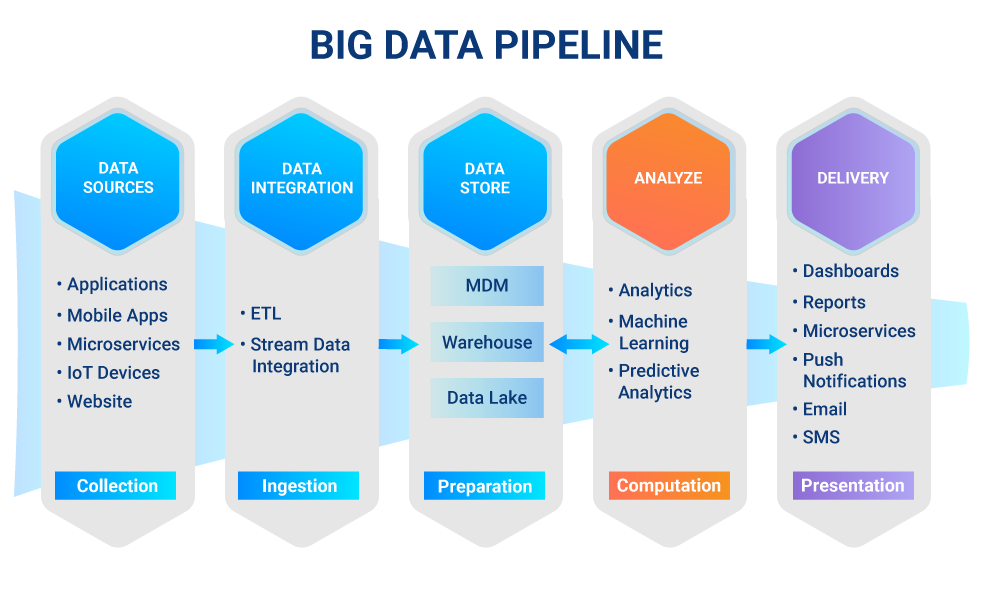
\includegraphics[width=\textwidth]{figures/pipeline.png}
    \caption{Layers of a Big Data pipeline~\cite{Davis2022}.}
    \label{fig:relatedwork-big-data-pipeline}
\end{figure}

In addition to the classic \ac{elt} steps, a modern data pipeline typically encompasses many more systematic aspects, as visualized in \cref{fig:relatedwork-big-data-pipeline}.
Often, a task orchestration solution such as the established \href{https://airflow.apache.org/}{\textit{Apache Airflow}} or the data movement platform \href{https://nifi.apache.org/}{\textit{Apache NiFi}} provides a \ac{gui} that allows analysis of data flow and lineage~\cite{Matskin2021, Faizan2021}.
For privacy reasons, regulations like the \ac{gdpr} require personally identifiable data to be anonymized or holistically removed from all data fragments and metadata accumulated in any part of the pipeline's data processing~\cite{Yu2016}.
Compliance rules can restrict permissions for interactions or mandate monitoring that sends notifications when abnormalities are detected.
Human configuration errors might necessitate the reprocessing of a certain amount of data, or scheduling logic might be needed to clean up outdated artifacts, such as extraneous files.
Optimizations such as partitioning, query caching, and data locality improvements can accelerate processing.
Finally, some pipelines use data version tagging or timestamping to enable jumps between specific versions of the stored data representation.

Batch processing pipelines existed even before the advent of reactive applications, which created the need for streaming pipelines.
Thus, streaming pipelines can be considered comparatively modern.
Although the objectives of this thesis do not include requirements for streaming capabilities, the streaming pipeline designs identified in our literature review on potential pipeline designs for our use case served as helpful inspiration and are briefly mentioned in this section.

\textbf{Aurangzaib et al.} (2022) published a scalable and containerized pipeline design based on \href{https://kafka.apache.org/}{\textit{Apache Kafka}}, \href{https://flink.apache.org/}{\textit{Apache Flink}}, and \href{https://cassandra.apache.org/}{\textit{Apache Cassandra}}.
This design is deployed on a \href{https://kubernetes.io/}{\textit{Kubernetes}} cluster for anomaly detection in \ac{iot} data~\cite{Aurangzaib2022}.
Kafka and Cassandra were also used by \textbf{Nazeer et al.} (2017) but connected through \href{https://spark.apache.org/}{\textit{Apache Spark}} instead of Flink for text analysis~\cite{Nazeer2017}.
\textbf{T and Chandrasekar} (2021) designed a pipeline system for telecommunication data processing using Kafka and Spark, with \href{https://www.elastic.co/de/elasticsearch}{\textit{ElasticSearch}} for storage~\cite{T2021}.
The approach by \textbf{Li and Zou} (2021) utilizes \ac{aws} as a cloud-based alternative to the Apache open source tools mentioned thus far, also for \ac{iot} sensor data processing, specifically anomaly detection~\cite{Li2021}.
Anomalies were also detected on massive production logs by \textbf{Chen2014} (2014) using \href{https://storm.apache.org/}{\textit{Apache Storm}}, a framework purely offering streaming, whereas Flink also offers some batching features.
\textbf{Khlevna and Koval} (2022) compared many of the mentioned processing frameworks to identify the best tools for anomaly detection in Big Data~\cite{Khlevna2022}.
A more abstract solution specifically targeting heterogeneous execution environments was proposed by \textbf{Wu et al.} (2016) due to the fragmented options available for choosing open source tools~\cite{Wu2016}.

An interesting finding outside of scientific literature was a patent for \textit{Systems and Methods for Creating Modular Data Processing Pipelines} by \textbf{Cha et al.} (2021), representatives of \textit{Pulsedata Inc}, an \ac{ai} healthcare company~\cite{Cha2021}.
The need for such a healthcare Big Data system is supported by the statement that existing \acp{gui} for medical applications already allow data sources to be tapped and combined, though these solutions lack Big Data capability.
Therefore, this patent does not appear to cover a general method for creating Big Data pipelines.


\subsubsection{Data Sources}
\label{sec:related-work-big-data-datasets}

Datasets fitting our use case of web data analysis are publicly available or can be sourced through crawling.
In both cases, some restrictions may apply, such as rate limiting for data pulls or denial of access for crawlers.

The \href{https://httparchive.org/}{\textit{HTTP Archive}} crawls around 15 million \acp{url} taken from the \href{https://developer.chrome.com/docs/crux}{\ac{crux}} each month.
Crawls by the HTTP Archive use \href{https://w3c.github.io/web-performance/specs/HAR/Overview.html}{\ac{har}} files generated by \href{https://developer.chrome.com/docs/lighthouse/}{\textit{Lighthouse}} for storing information about page access in the human-readable \ac{json} format.
The HTTP Archive's dataset is available publicly on the \ac{gcp}.

Annually, the HTTP Archive aims to publish the \href{https://almanac.httparchive.org/}{\textit{Web Almanac}}, a report on the state of the web.
The Web Almanac's 2022 edition is the most recent at the time of writing and includes 23 chapters about page contents, \ac{ux} metrics, content publishing, and content distribution.

Other sources for \acp{url} are the \ac{dns}-sourced \href{https://radar.cloudflare.com/domains}{\textit{Cloudflare Radar} domain ranking}, the user access monitoring-sourced \href{https://s3-us-west-1.amazonaws.com/umbrella-static/index.html}{\textit{Cisco Umbrella} popularity list}, and the subnet-sourced \href{https://majestic.com/reports/majestic-million}{\textit{Majestic Million}}.
Up until its end of service in 2021, a commonly known source for a top-1-million dataset was provided by \textit{Alexa Internet, Inc.}.

A public dataset of more than 250 billion pages is provided by \href{https://commoncrawl.org/}{\textit{Common Crawl}}, a non-profit founded in 2007.
New data is added to Common Crawl's corpus monthly and is freely accessible thanks to the \textit{Open Data Sets Sponsorship} by \ac{aws}.
The most recent dataset at the time of writing is the October 2024 dataset (\texttt{CC-MAIN-2024-42}), which includes 2.49~billion pages amounting to 365~TiB of uncompressed content spanning 47.5~million hosts and 38.3~million domains~\cite{Vaughan2024}.
The datasets can be accessed within \ac{aws} using the \ac{aws} \ac{cli} or via \ac{http}.

Current monthly Common Crawl data is formatted as \ac{warc}, \ac{wat}, and \ac{wet} files and also includes \texttt{ro\-bots\-.txt} results, results that returned a non-successful status code, and a \ac{url} index in row- and column-based style.
\ac{warc} files include the raw data crawled, including metadata on \ac{http} requests and responses and on the crawl process itself.
In \ac{wat} files, the full metadata for a crawl can be accessed in \ac{json} format.
The \ac{wet} files include only plaintext extracted from a crawled page.

Nine hundred such files make up a segment, and a monthly Common Crawl includes 100 segments.
In the most recent crawl, the compressed sizes are 77.33~TiB for \ac{warc} files, 17.33~TiB for \ac{wat} files, and 6.87~TiB for \ac{wet} files.
The \texttt{robots.txt} data has a size of 0.14~TiB, and non-\texttt{200} responses amount to 2.49~TiB.
The \ac{url} index occupies 0.19~TiB in row-based and 0.22~TiB in columnar format.

Common Crawl provides \href{https://commoncrawl.github.io/cc-crawl-statistics/}{statistical analyses of their crawls} that we can inspect now and compare to our own results later in \cref{sec:evaluation}.
The statistics include the following data on the crawl \texttt{CC-MAIN-2024-42}:

\begin{enumerate}
    \item \acp{cctld} make up 43.22\% of the dataset, spanning 1,077,971,520 pages and 19,309,814 hosts.
    \item \texttt{.ru} and \texttt{.de} are the most common \acp{cctld} with 4.6\% and 3.95\% shares, respectively, only surpassed by the \texttt{.com} and \texttt{.org} \acp{tld} with 42.51\% and 5.59\% shares.
    \item \texttt{blogspot.com} and \texttt{wikipedia.org} host the most pages: 14,995,155 and 4,995,736, respectively.
    \item \texttt{UTF-8} is the predominant charset with a share of 93.3\%.
    \item \texttt{Language detection} by \href{https://github.com/CLD2Owners/cld2}{\textit{Compact Language Detector 2}} found English to be the most common language, with a 43.4\% share, and Russian to be the second most common language, with a 6\% share.
\end{enumerate}

The \ac{ua} used by Common Crawl is named \textit{CCBot} and identifies as an \href{https://nutch.apache.org/}{\textit{Apache Nutch}}-based crawler that relies on \href{https://hadoop.apache.org/}{\textit{Apache Hadoop}} for ``distributed processing of large data sets across clusters of computers''.
Besides Nutch, other commonly used tools for web scraping include \href{https://www.crummy.com/software/BeautifulSoup/}{\textit{BeautifulSoup}}, \href{https://scrapy.org/}{\textit{Scrapy}}, and \href{https://www.selenium.dev/}{\textit{Selenium}}.
While BeautifulSoup is primarily a parsing library, Scrapy is tailored towards web scraping with features like asynchronous requests and politeness towards scraped web servers.
Selenium is a browser automation engine, which is a major benefit for scraping pages that block non-human-like access patterns.

Fighting anti-crawler protection measures can be challenging, depending on the level of protection a server has implemented.
Services like \href{https://www.cloudflare.com/}{\textit{Cloudflare}} execute \ac{js} code to detect a browser environment and can exclude simple \ac{http} clients from accessing a \ac{url}.
If \ac{js} cannot be executed, which is a valid environment even for human access, as browsers allow disabling \ac{js} for security reasons, Cloudflare shows a CAPTCHA.
There are CAPTCHA-solving services like \href{https://deathbycaptcha.com/}{\textit{Death By Captcha}}, but requests coming from \ac{ip} ranges known to be owned by major cloud providers are often blocked by default.
Running crawls on infrastructure on personal machines would be an alternative to cloud providers, but if one's own \ac{ip} addresses are blacklisted, it is often not as trivial to change the \ac{ip} address as it is with cloud providers.

With all scraping, politeness rules dictate that the crawler's access patterns should not burden the servers accessed.
Data protection regulations like the \ac{gdpr} should be respected, and personally identifiable information should not be stored.
Concurrent requests to a page should be limited and possibly even sent during times of low organic load by human users~\cite{Patel2020}.
